\documentclass{anstrans}
%%%%%%%%%%%%%%%%%%%%%%%%%%%%%%%%%%%
\title{An Approach for Load Balancing Massively Parallel Transport Sweeps on Unstructured Grids}
\author{Tarek H. Ghaddar, Jean C. Ragusa}

\institute{
Dept. of Nuclear Engineering, Texas A\&M University, College Station, TX, 77843-3133
\and

}

\email{tghaddar@tamu.edu \and jean.ragusa@tamu.edu}

%%%% packages and definitions (optional)
\usepackage{color} 
\usepackage{graphicx} % allows inclusion of graphics
\usepackage{booktabs} % nice rules (thick lines) for tables
\usepackage{microtype} % improves typography for PDF
%Math Symbols
\newcommand{\vr}{\vec{r}}
\newcommand{\vo}{\vec{\Omega}}
%Allows [H] option
\usepackage{float}
%Allow page breaks within align
\allowdisplaybreaks
%Allows for easy pseudocode.
\usepackage{listings}
%Changing spacing in itemized lists
\usepackage{enumitem}
\setlist{nosep}
%Include a pdf file
\usepackage{pdfpages}
%Eps figures
\usepackage{epstopdf}
%Algorithm
\usepackage{algorithm}
\usepackage{algorithmic}

\newcommand{\SN}{S$_N$}
\renewcommand{\vec}[1]{\bm{#1}} %vector is bold italic
\newcommand{\vd}{\bm{\cdot}} % slightly bold vector dot
\newcommand{\grad}{\vec{\nabla}} % gradient
\newcommand{\ud}{\mathop{}\!\mathrm{d}} % upright derivative symbol
\newcommand{\tcr}[1]{\textcolor{red}{#1}} % upright derivative symbol

\begin{document}
%%%%%%%%%%%%%%%%%%%%%%%%%%%%%%%%%%%%%%%%%%%%%%%%%%%%%%%%%%%%%%%%%%%%%%%%%%%%%%%%
\section{Introduction}
\label{ch:introduction}
When running any massively parallel code, attaining load balancing is a priority in order to achieve the best possible parallel efficiency. A load balanced problem has an equal number of degrees of freedom per processor. Load balancing is an important factor to minimize idle time for all processors and is attained by equally distributing (as much as possible) the work load among all processors. 
% This makes communicating information in between processors more efficient, improving parallel efficiency. 

To the best of our knowledge, transport sweeps are the only method to scale on current and next-generation supercomputers. PDT, Texas A\&M University's massively parallel deterministic transport code, has been shown to scale on logically Cartesian grids out to 750,000 cores \cite{mpadams2015}. Logically Cartesian grids are constructed with mesh cells that are identified using integer triplets $ijk$ (i.e., cubic cells), but allow for vertex motion in order to conform to curved shapes. The concepts and results presented in this paper are implemented in PDT. PDT is a solver for neutron, thermal, gamma, coupled neutron-gamma, electron, and coupled electron-photon radiation transport phenomena. It uses discrete ordinates for angular discretization, multi-group data, and discontinuous finite elements in space. 

A new unstructured meshing capability was implemented in PDT in order to realistically represent certain geometries. Cut lines (planes for 3D cases) are used to partition such geometries into logically-Cartesian subdomains, which are then individually meshed in parallel using the Triangle Mesh Generator \cite{triangle}. These subdomains are then "stitched" together in order to create a continuous geometry. 2D meshes can be extruded in the $z$ dimension for 3D problems. 

However, unstructured meshes often create unbalanced problems due to the way localized features are meshed, so a load balancing algorithm was added into PDT. 

% A load balanced problem is determined by the value of $f$, where $f$ is the subset with the maximum number of cells, divided by the average number of cells per subset. A perfectly balanced problem has $f = 1$.


%%%%%%%%%%%%%%%%%%%%%%%%%%%%%%%%%%%%%%%%%%%%%%%%%%%%%%%%%%%%%%%%%%%%%%%%%%%%%%%%


%%%%%%%%%%%%%%%%%%%%%%%%%%%%%%%%%%%%%%%%%%%%%%%%%%%%%%%%%%%%%%%%%%%%%%%%%%%%%%%%
\section{Application of 2D and 3D Unstructured Meshes}
\label{ch:motivation}

The capability for PDT to generate and run using unstructured meshes is important because it enables more realistic problems to be tackled. However, we wish to preserve a logically-Cartesian grid at the "subset" level, with an unstructured mesh inside each subset. These logically Cartesian subdomains (subsets) are obtained using cut planes in 3D and cut lines in 2D. Figure \ref{grid} demonstrates this functionality. The geometry is decomposed into 3 subsets in $x$ and 3 in $y$, with the first two subsets meshed using Triangle.

\begin{figure}[H]
\centering
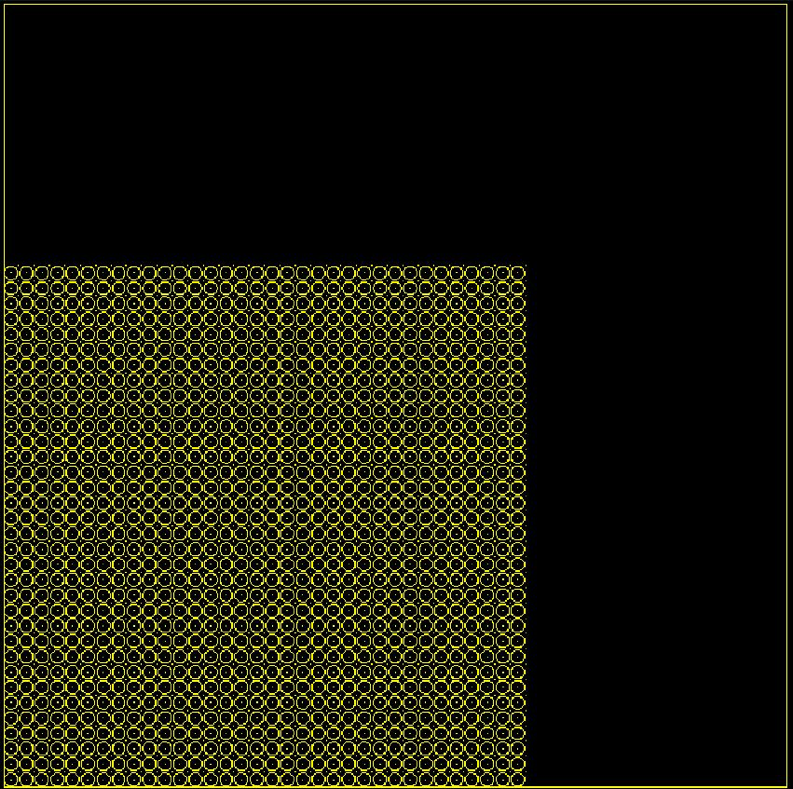
\includegraphics[scale = 0.45]{figures/lattice.png}
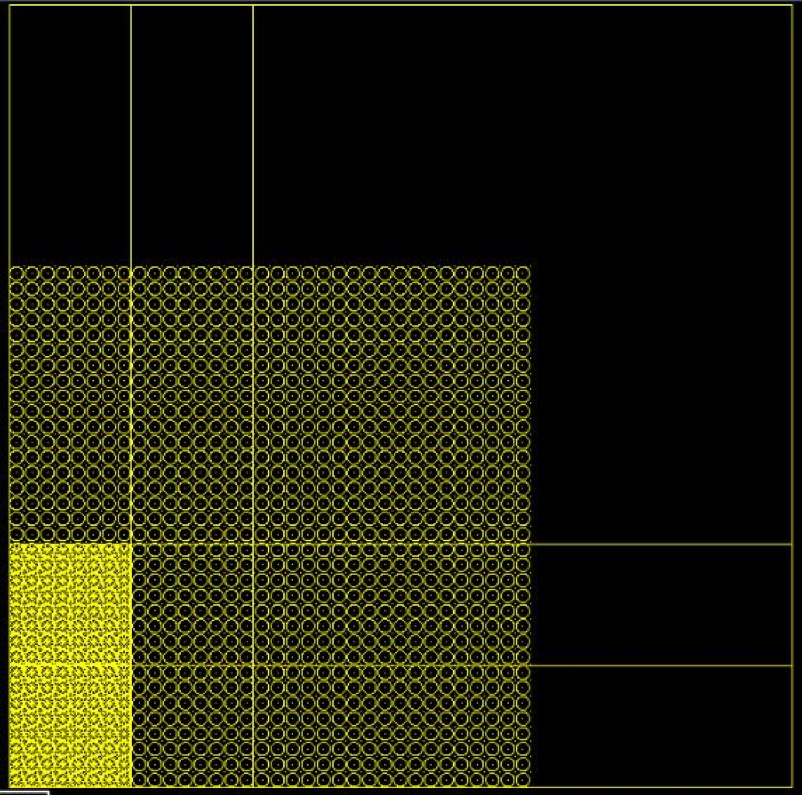
\includegraphics[scale = 0.45]{figures/subsetlattice.png}
\caption{A PSLG describing a fuel lattice (top image), and the ``subset" grid imposed on the PSLG (bottom image, with only 2 subsets meshed for illustration purposes).}
\label{grid}
\end{figure}

The orthogonal grid composed of the cut planes is superimposed on the geometry; each resulting subset is meshed in parallel.  Subsets are now the base structured unit when performing transport sweeps. Discontinuities along the subset boundary are fixed by "stitching'' hanging nodes, creating degenerate polygons along these boundaries. Because PDT's spatial discretization employs Piece-Wise Linear Discontinuous (PWLD) finite element basis functions, degenerate polygons do not lead to numerical difficulties at the local cell solve. \cite{pwld_teresa,pwld_ragusa}.

Currently, only 2D and 2D extruded unstructured capability is available in PDT. The 2D input geometry is described by a Planar Straight Line Graph (PSLG). After superimposing the orthogonal grid, a PSLG is created for each subset, and meshed. The mesh can be extruded in the $z$ dimension for 3D problems. Obviously, this is not as general as a 3D unstructured tetrahedral mesh, but for many problems of interest, it is a useful capability to have. Furthermore, this simpler setting allows for the testing of our load balancing approach for unstructured grids.

To demonstrate the newly implemented unstructured meshing capability in PDT, Texas A\&M Nuclear Engineering's Impurity Model 1 (IM1) problem is used. Figure \ref{IM12D} showcases the 2D mesh of the IM1 problem,

\begin{figure}[H]
\centering
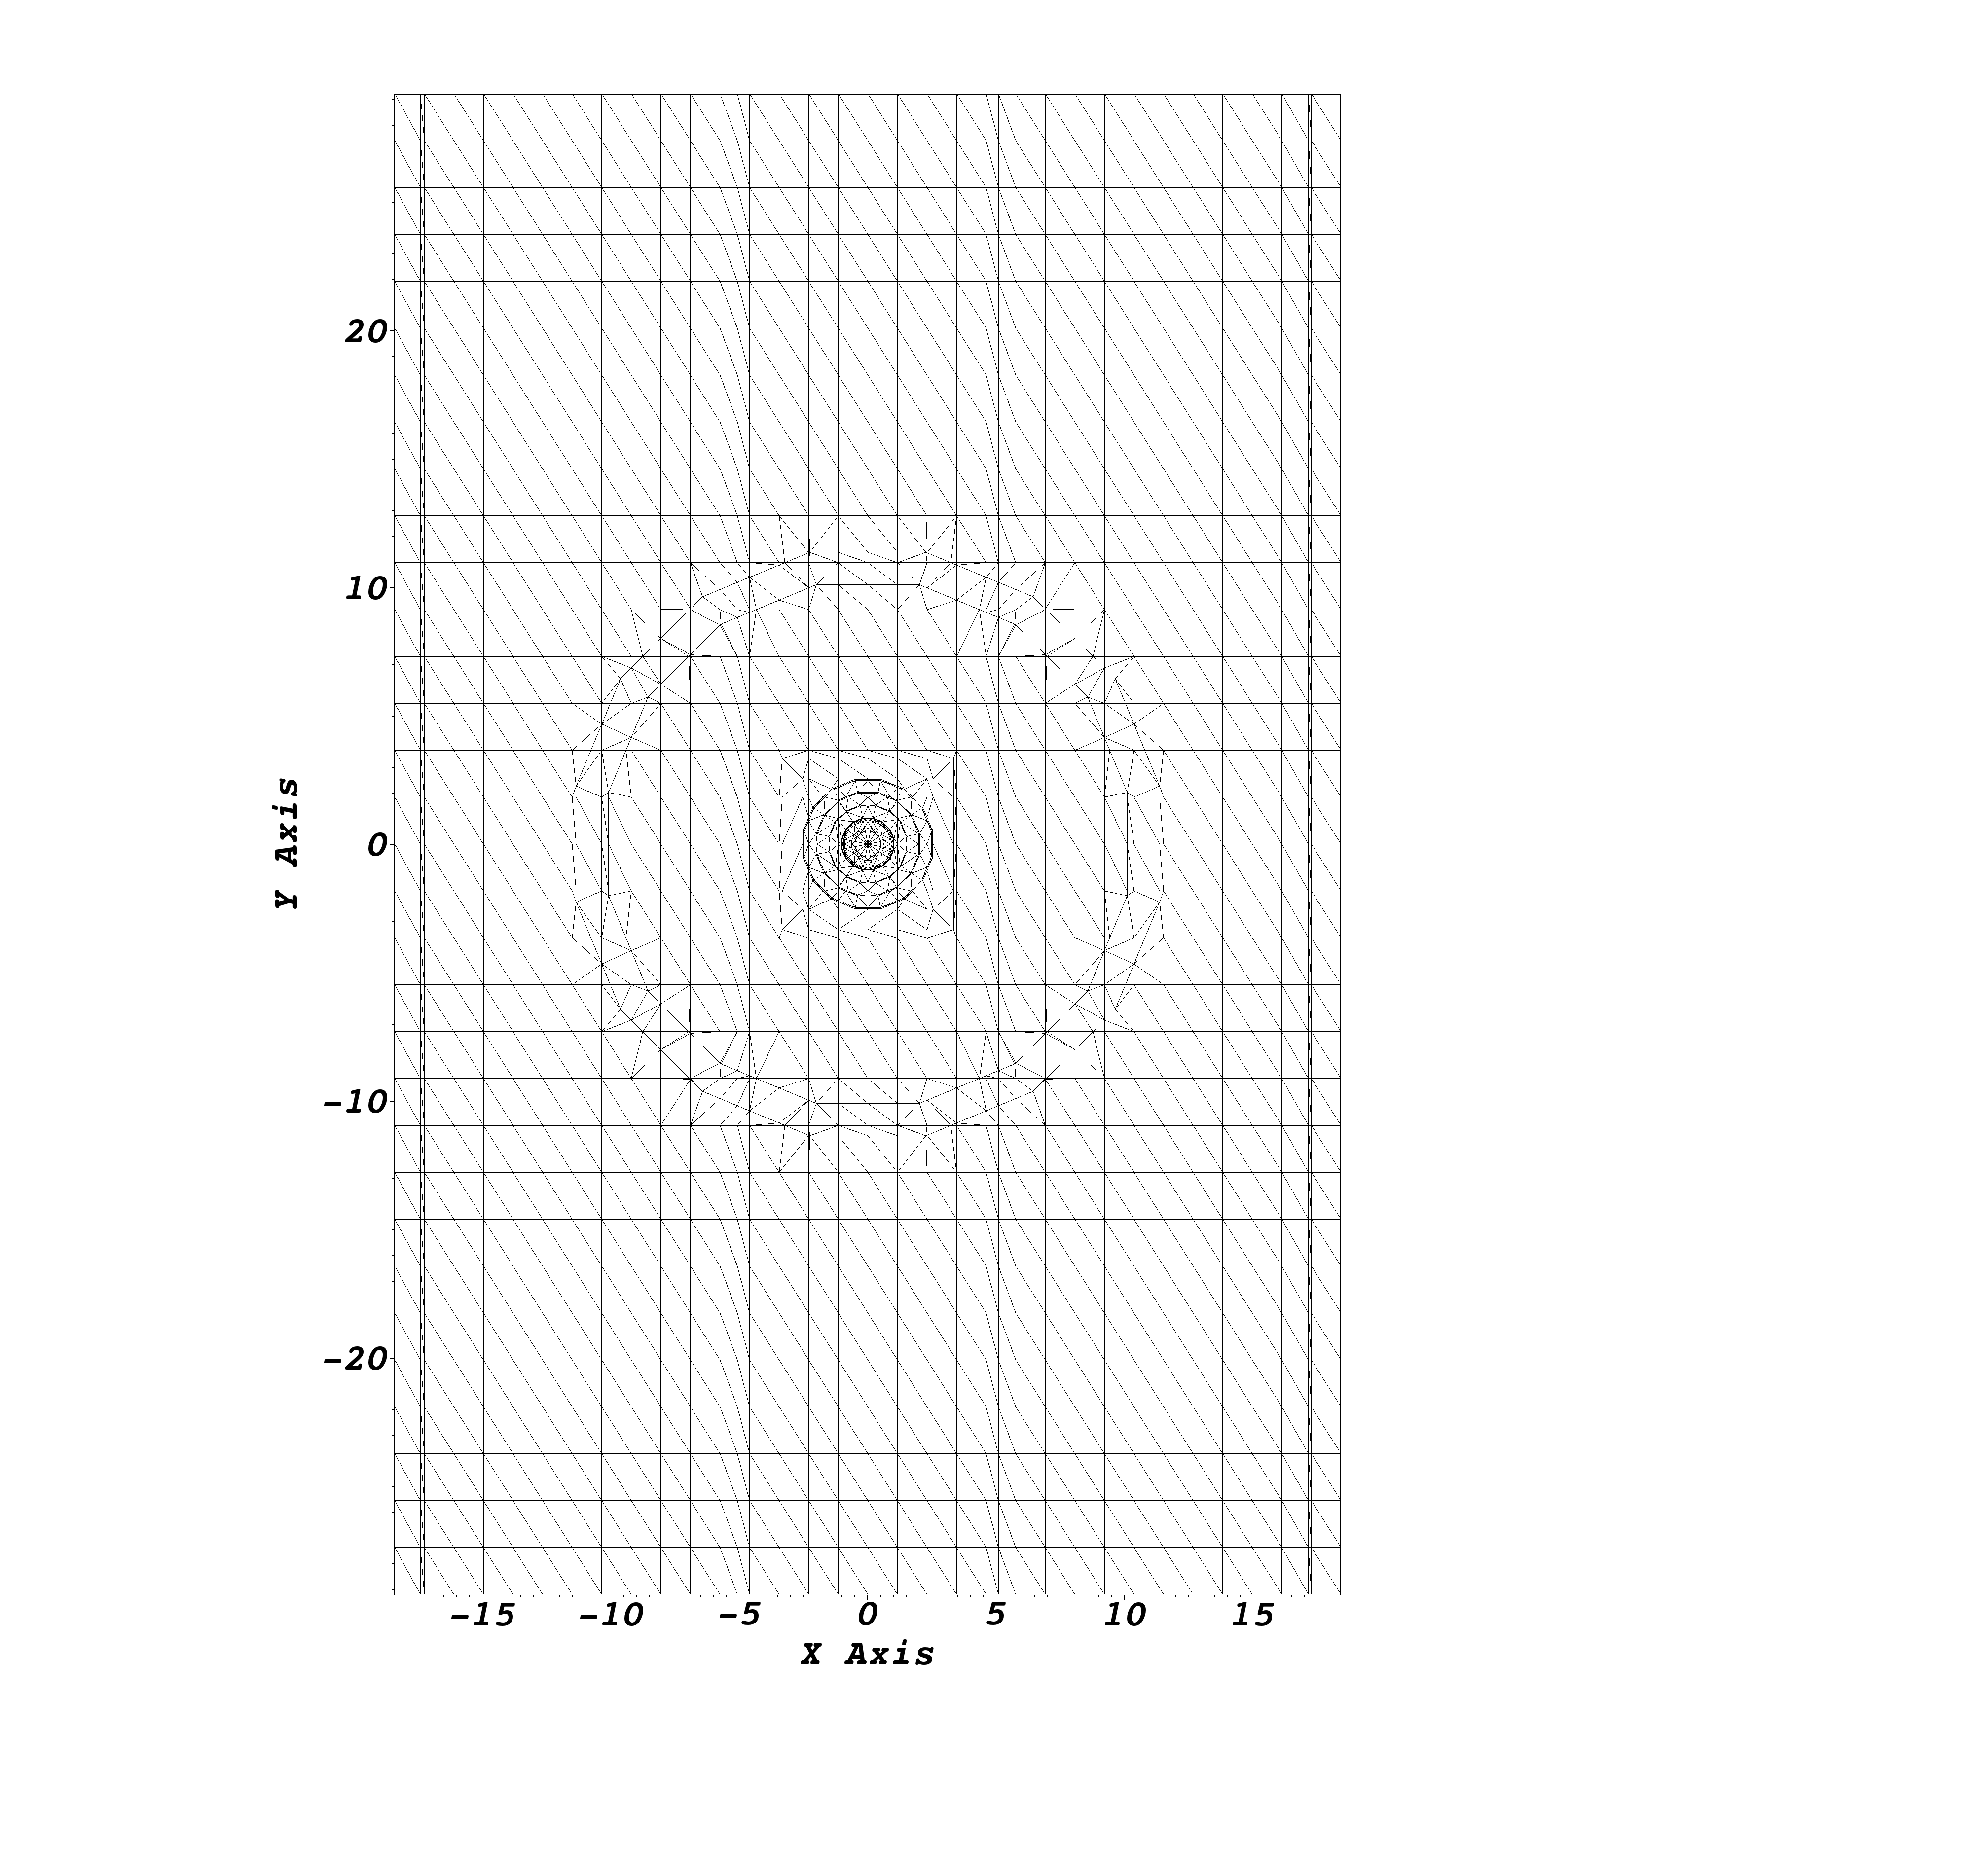
\includegraphics[scale = 0.13, trim=28cm  4cm 0cm 4cm,clip]{figures/im12d.png}
\caption{The 2D mesh of the IM1 problem.}
\label{IM12D}
\end{figure}

The combination of the 2D mesh and extrusion parameters yield the full 3D problem, shown in Fig. \ref{IM13D}.

\begin{figure}[H]
\centering
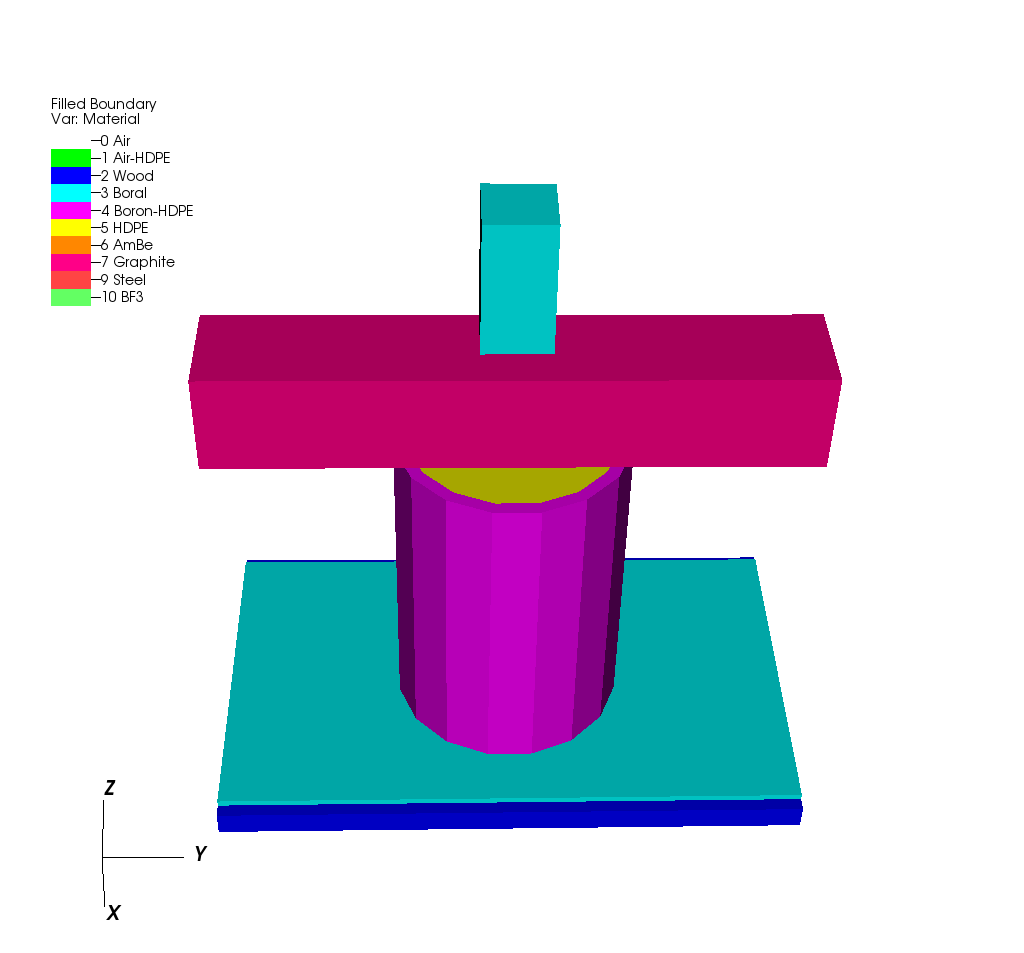
\includegraphics[scale = 0.3]{figures/IM1_3D.png}
\caption{The 2D extruded view of the IM1 problem.}
\label{IM13D}
\end{figure}


\section{The Load Balancing Algorithm}

If the number of cells in each subset can be reasonably balanced, then the problem is effectively load balanced. This has already been done using  the provably-optimal transport sweep algorithm on logically Cartesian grids \cite{mpadams2015}.  We extend this concept to unstructured meshes. The Load Balance algorithm described below details how the subsets will be load balanced. In summary, the procedure of the algorithm involves moving the initially user-specified $x$ and $y$ cut planes, re-meshing, and iterating until a reasonably load balanced problem is obtained.  The load balancing metric, shown in Equation~\eqref{metric_def}, dictates how balanced or unbalanced a problem is:
\begin{equation}
f =\frac{\underset{ij}{\text{max}}(N_{ij})}{\frac{N_{tot}}{I\cdot J}},
\label{metric_def}
\end{equation}
where $f$ is the load balance metric, $N_{ij}$ is the number of cells in subset $i,j$, $N_{tot}$ is the global number of cells in the problem, and $I$ and $J$ are the total number of subsets in the $x$ and $y$ direction, respectively. The metric is a measure of the maximum number of cells per subset divided by the average number of cells per subset.

The load balancing algorithm moves cut planes based on two sub-metrics, $f_I$ and $f_J$. Equation ~\eqref{submetric} defines these two parameters:
\begin{subequations}
\label{submetric}
\begin{equation}
f_I = \frac{ \underset{i}{\text{max}}[\sum_{j} N_{ij}] } {\frac{N_{tot}}{I}} 
\end{equation}
\begin{equation}
f_J = \frac{\underset{j}{\text{max}}[\sum_{i} N_{ij}] } {\frac{N_{tot}}{J}}.
\end{equation}
\end{subequations}
%
$f_I$ is calculated by taking the maximum number of cells per column and dividing it by the average number of cells per column. $f_J$ is calculated by taking the maximum number of cells per row and dividing it by the average number of cells per row. If these two numbers are greater than predefined tolerances, the cut lines in the respective directions are redistributed. Once redistribution and remeshing occur, a new metric is calculated. This iterative process occurs until a maximum number of iterations is reached, or until $f$ converges within the user defined tolerance. The Load Balance algorithm behaves as follows:

\lstinputlisting[language = C++, basicstyle = \footnotesize]{loadbalance.cc}

%%%%%%%%%%%%%%%%%%%%%%%%%%%%%%%%%%%%%%%%%%%%%%%%%%%%%%%%%%%%%%%%%%%%%%%%
\section{Results}
\label{ch:results}

The following sections will showcase the metric behavior and convergence for three test cases and the new unstructured meshing capability both in 2D and 3D.

\subsection{Test Cases for Metric Behavior and Convergence}
\label{sec:convergence}
In order to illustrate the behavior of the load balancing metric, calculated by Eq.\ref{metric_def}, two test cases are presented. Figure \ref{opp} shows the first test case, a 20 cm by 20 cm domain with two pins in opposite corners of the domain. This is a theoretically very unbalanced case, as geometrically there are two features located distantly from each other with an empty geometry throughout the rest of the domain. Figure \ref{lattice} shows a lattice and reflector, which due to its denser and repeated geometry, theoretically is a more balanced problem. One more test case will be presented in the full paper.

A series of 162 inputs was constructed for each case. These inputs are constructed by varying the maximum triangle area from the coarsest possible to 0.01 cm\textsuperscript{2}. In addition, the number of subsets, $N$, varies from 2$\times$2 to 10$\times$10. 

\begin{figure}[H]
\centering
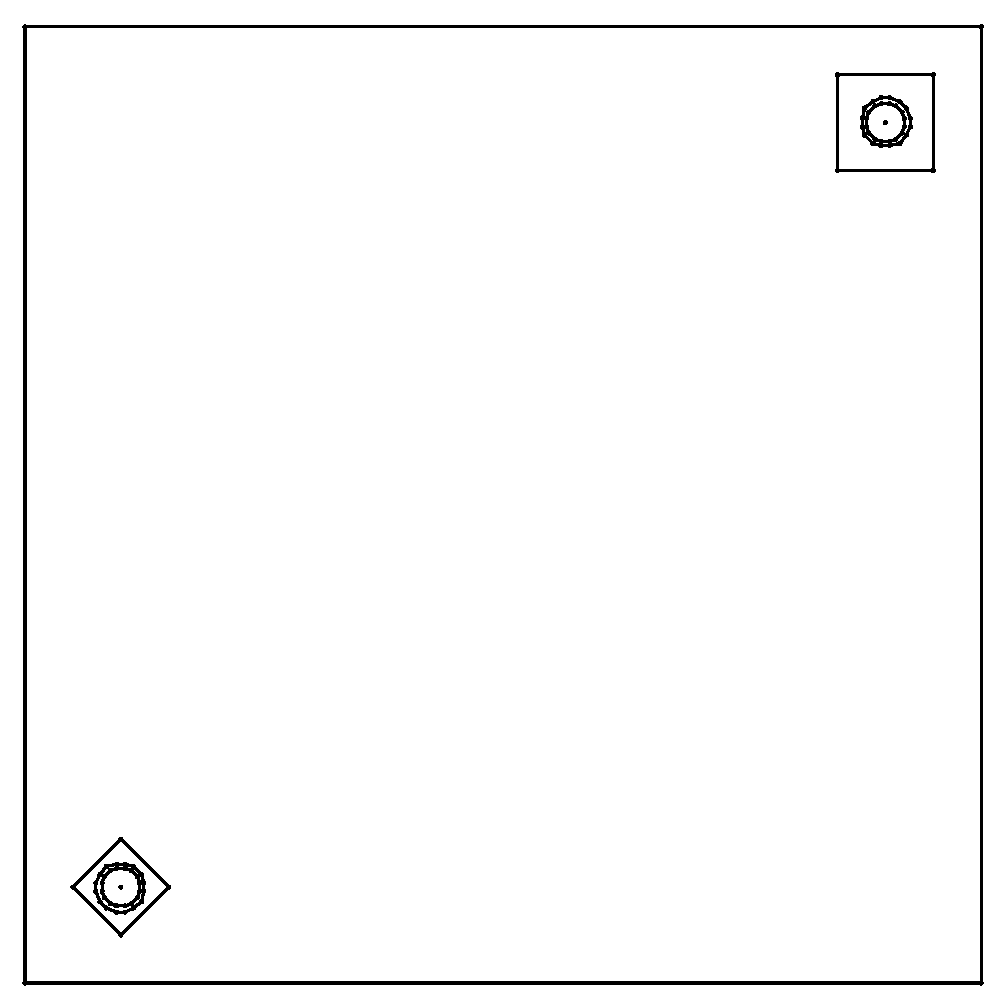
\includegraphics[scale = 0.5,trim = {0, 0, 0, 0}, clip]{figures/unbalanced_lattice.eps}
\caption{The first test case used in order to test effectiveness and convergence of the load balancing metric.}
\label{opp}
\end{figure}

\begin{figure}[H]
\centering
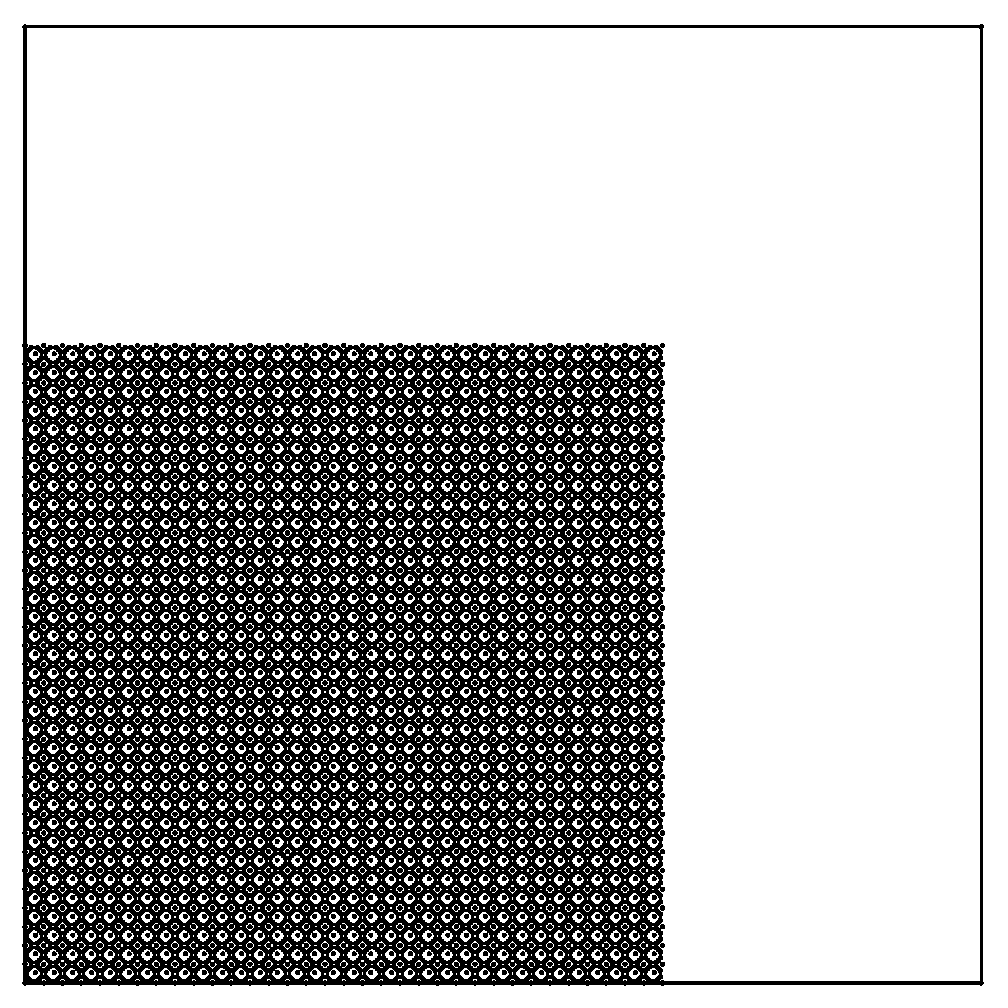
\includegraphics[scale = 0.5]{figures/lattice-12-shifted.eps}
\caption{The third test case used in order to test effectiveness and convergence of the load balancing metric.}
\label{lattice}
\end{figure}

\subsection{Metric Behavior and Convergence}

For each test case, the 162 input inputs are run twice, once with no load balancing iterations, and once with ten load balancing iterations. The best metric is reported and recorded. Two figures for each test cases are presented below: the first figure will show the metric behavior for no iterations and the second figure will show the metric behavior for each input run with ten load balancing iterations.

Figure \ref{oppnoiter} shows the metric behavior for Fig. \ref{opp}. The maximum metric value is 24.7650, and occurs when Fig. \ref{opp} is run with 8x8 subsets and a maximum triangle area of 1.6 cm\textsuperscript{2}. The minimum metric value is 1.0016 and occurs when Fig. \ref{opp} is run with 4x4 subsets and a maximum triangle area of 0.04 cm\textsuperscript{2}. 

\begin{figure}[H]
\centering
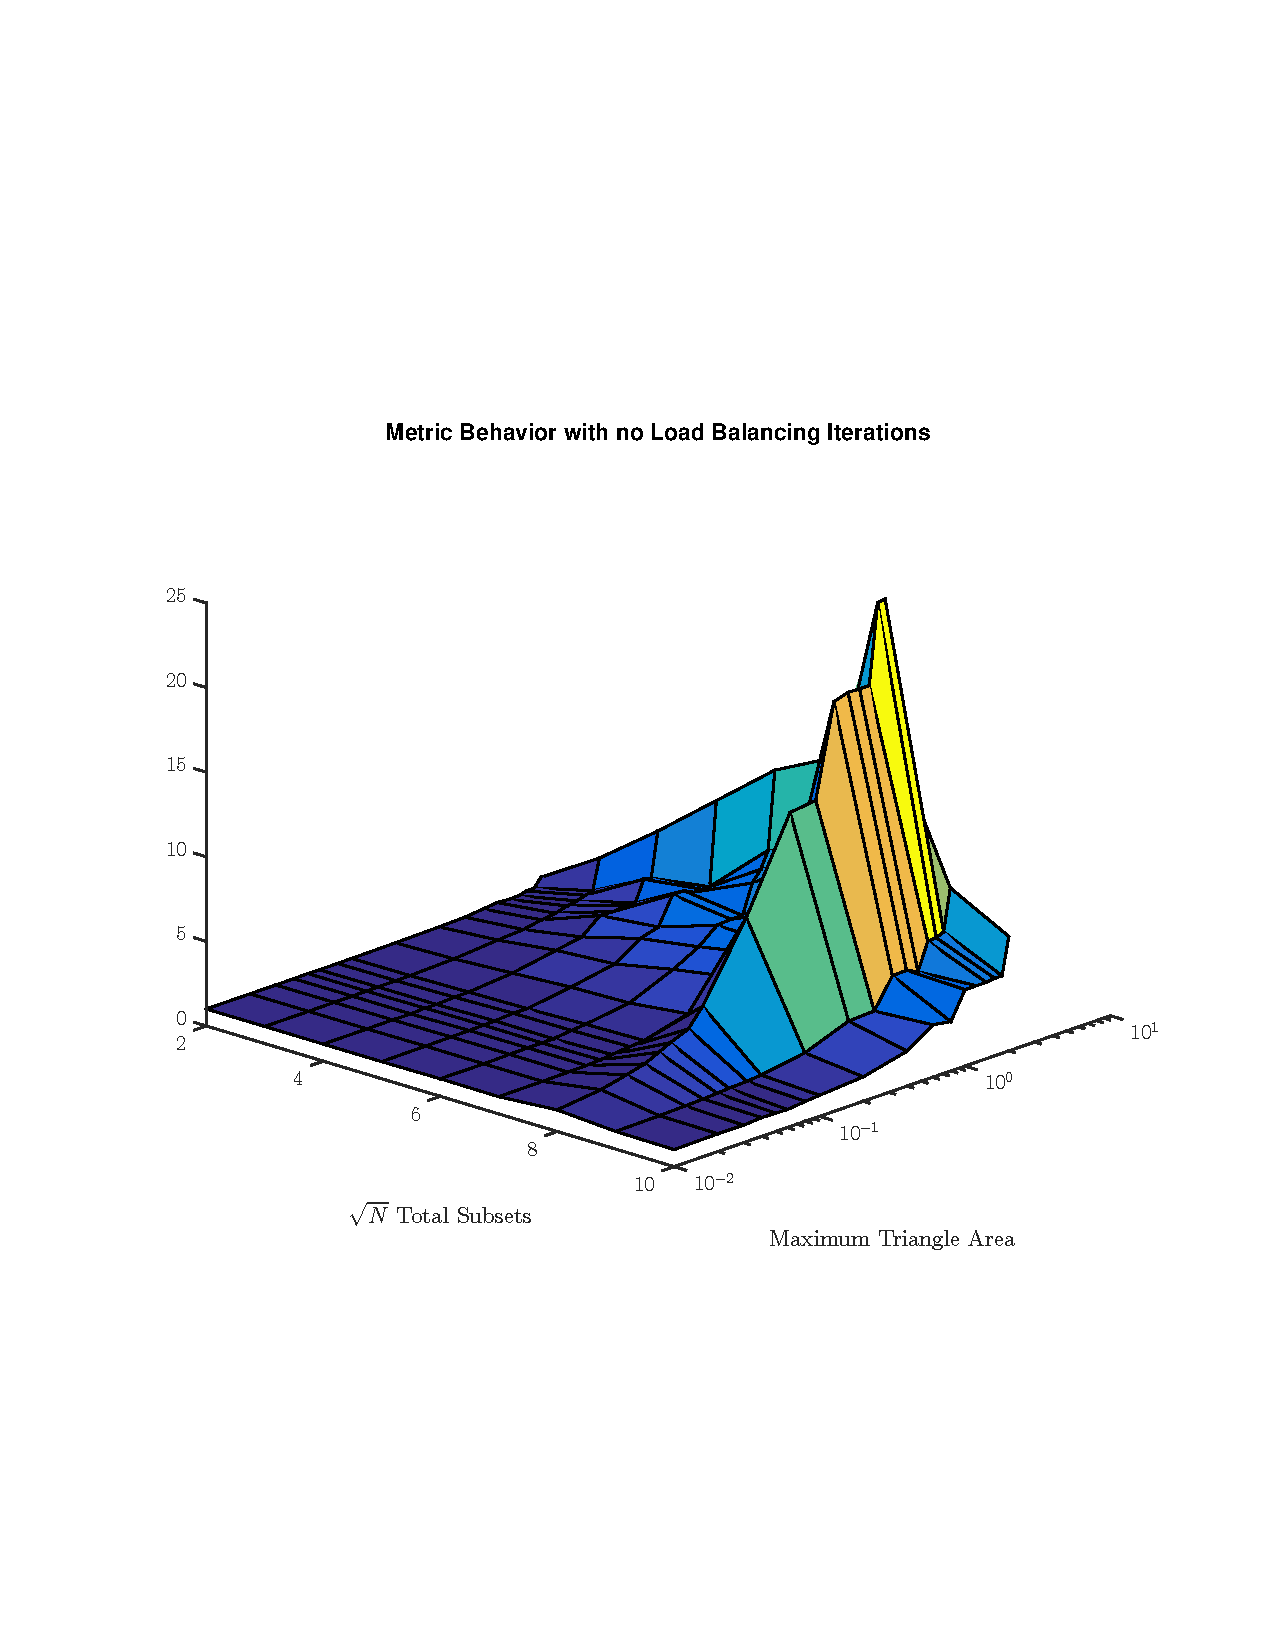
\includegraphics[scale=0.5, trim = 0cm 8cm 0cm 7cm,clip]{figures/OppNoIter.pdf}
\caption{The metric behavior of the first test case run with no load balancing iterations.}
\label{oppnoiter}
\end{figure}

Figure \ref{oppiter} shows the metric behavior for Fig. \ref{opp} after 10 load balancing iterations. The maximum metric value is 5.0538 and occurs when Fig. \ref{opp} is run with 10x10 subsets and a maximum triangle area of 1.2 cm\textsuperscript{2}. The minimum metric value is 1.0017 and occurs when Fig. \ref{opp} is run with 4x4 subsets and a maximum triangle area of 0.04 cm\textsuperscript{2}.

\begin{figure}[H]
\centering
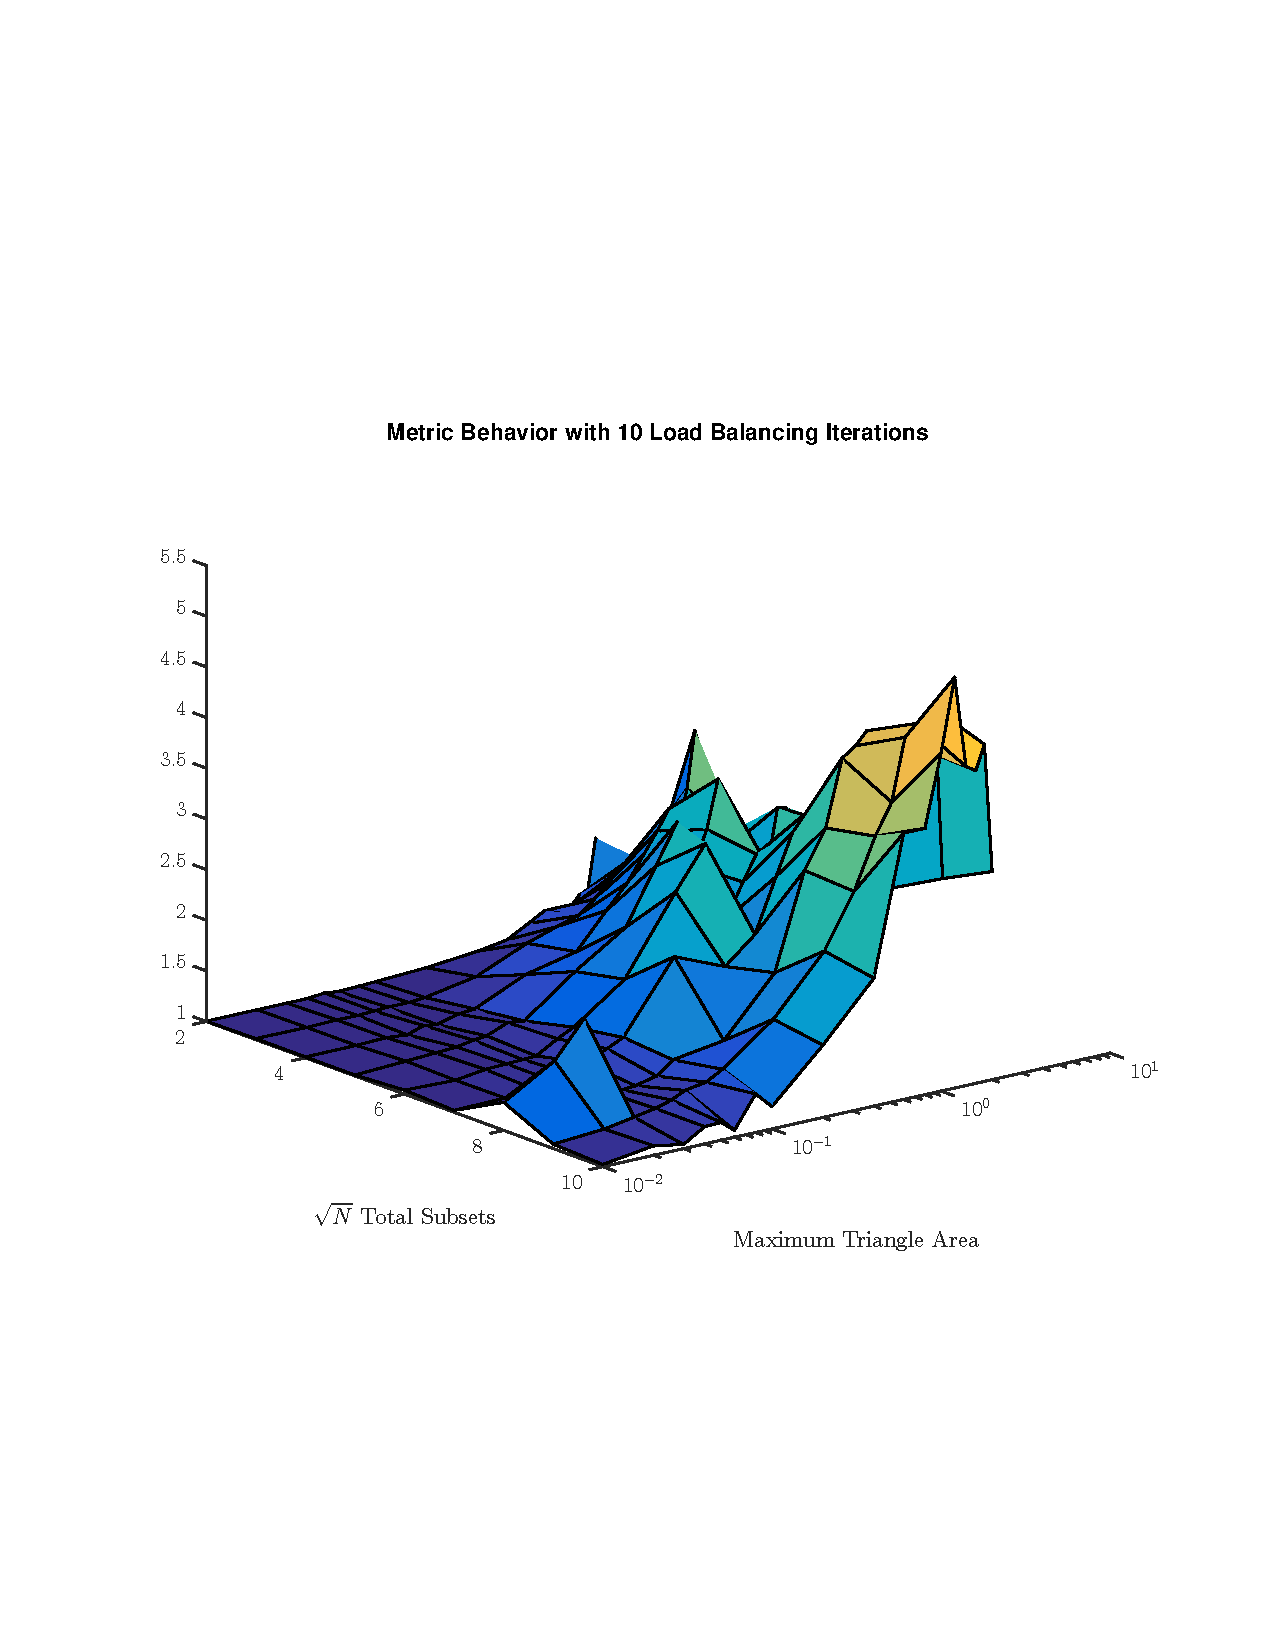
\includegraphics[scale=0.5, , trim = 2cm 6cm 2cm 7cm,clip]{figures/OppIter.pdf}
\caption{The metric behavior of the first test case run with 10 load balancing iterations.}
\label{oppiter}
\end{figure}

Figure \ref{latticenoiter} shows the metric behavior for Fig. \ref{lattice}. The maximum metric is 2.6489 and occurs when Fig. \ref{lattice} is run with 10x10 subsets with a maximum triangle area of 1.8 cm\textsuperscript{2}. The minimum metric is 1.0179 and occurs when Fig. \ref{lattice} is run with 2x2 subsets with a maximum triangle are of 0.08 cm\textsuperscript{2}.

\begin{figure}[H]
\centering
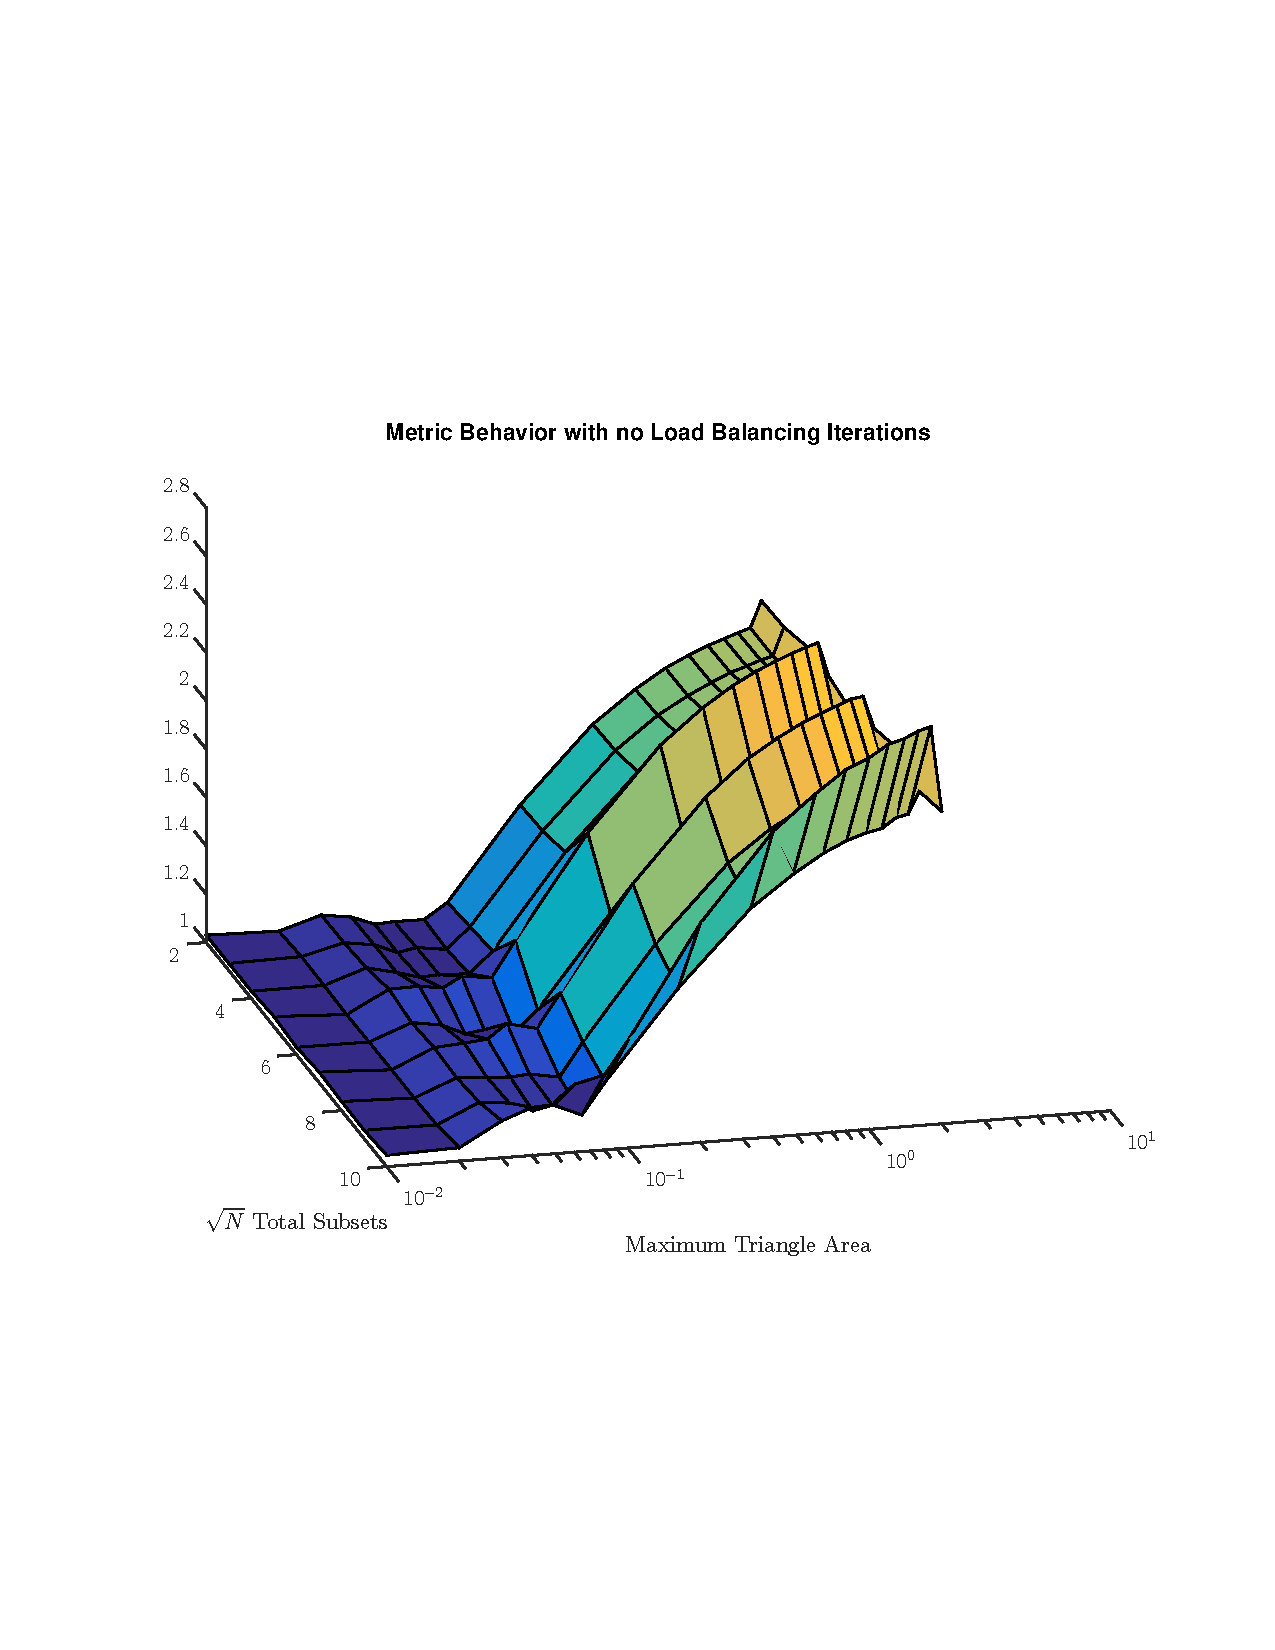
\includegraphics[scale=0.50, trim = 2cm 6cm 2cm 7cm,clip]{figures/lattice_no_iter.pdf}
\caption{The difference in metric behavior of the third test case with no load balancing iterations.}
\label{latticenoiter}
\end{figure}

Figure \ref{latticeiter} shows the metric behavior for Fig. \ref{lattice} after ten load balancing iterations. The maximum metric is 2.2660 and occurs when Fig. \ref{lattice} is run with 10x10 subsets with a maximum triangle area of 0.4 cm\textsuperscript{2}. The minimum metric is 1.0021 and occurs when Fig. \ref{lattice} is run with 2x2 subsets with the Triangle's coarsest possible mesh.

\begin{figure}[H]
\centering
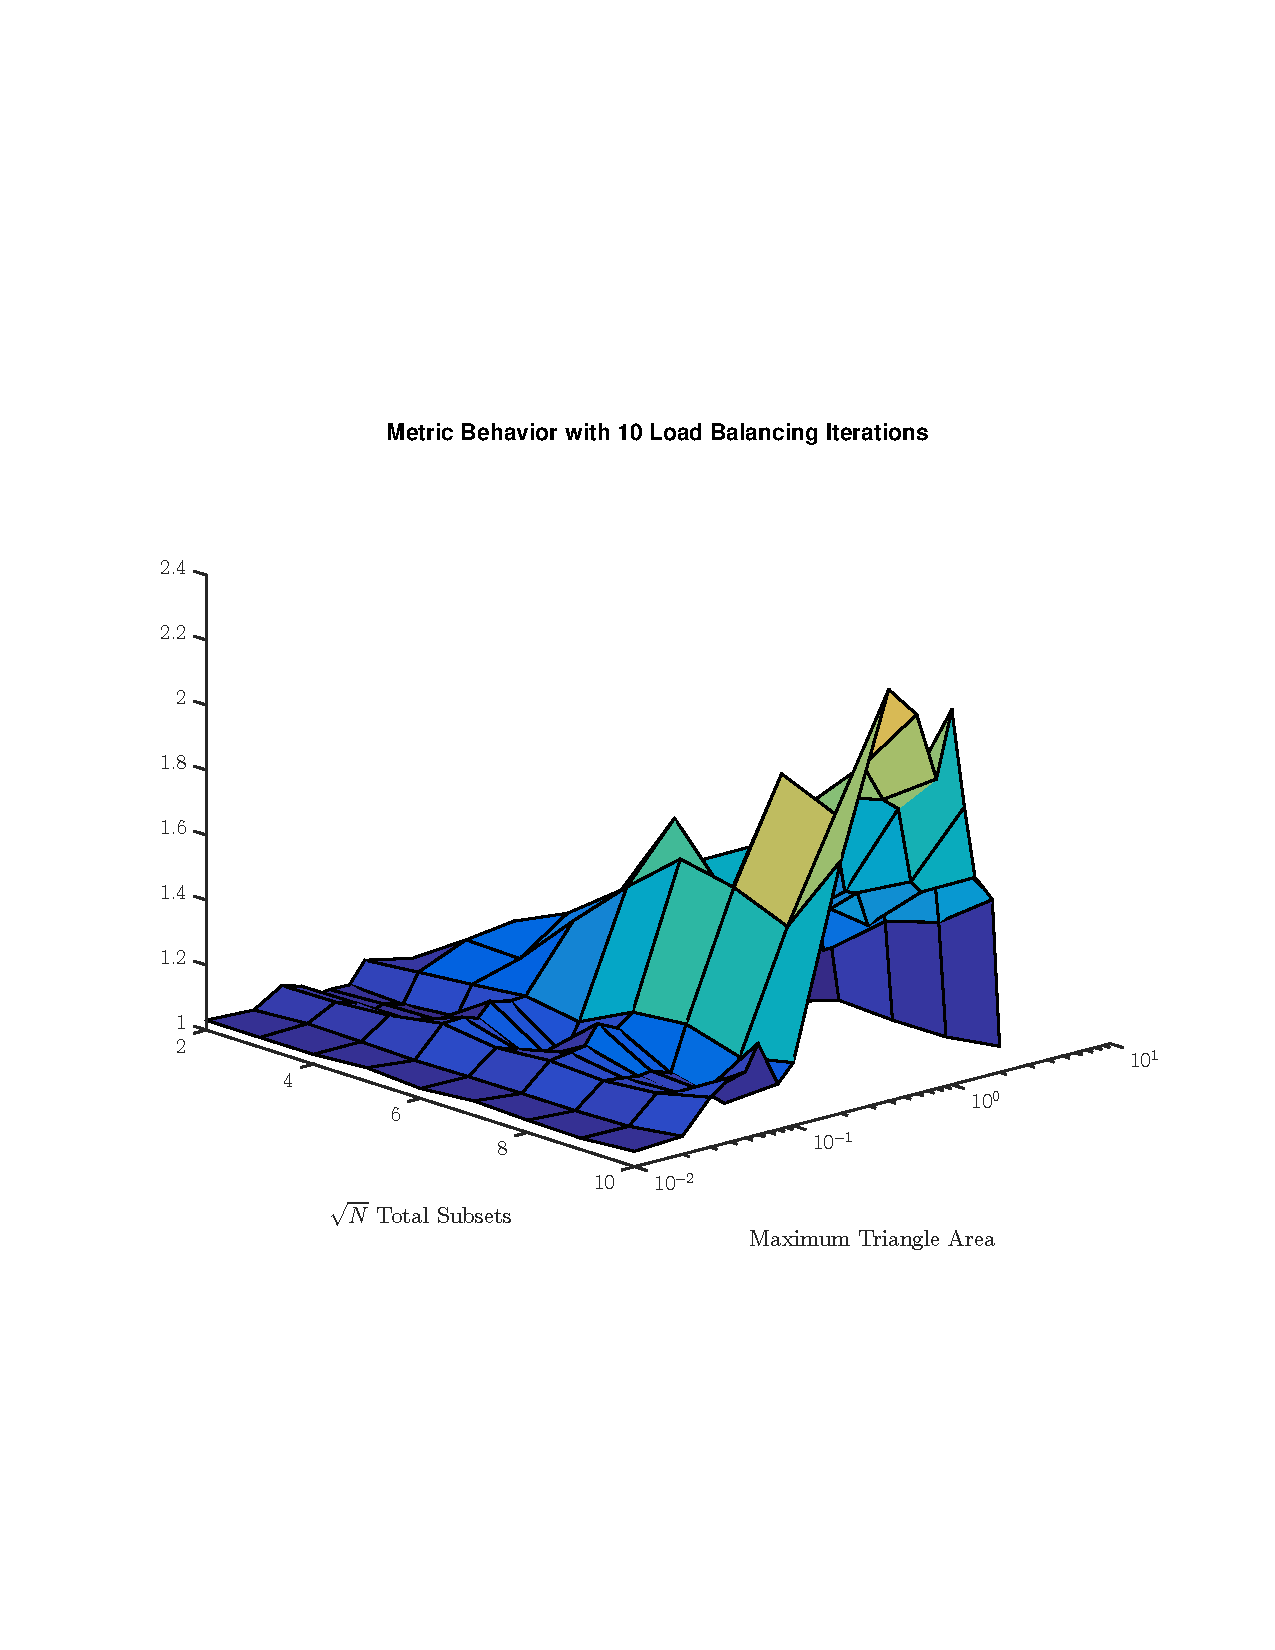
\includegraphics[scale=0.5, trim = 2cm 6cm 2cm 7cm,clip]{figures/lattice_iter.pdf}
\caption{The difference in metric behavior of the third test case after ten load balancing iterations.}
\label{latticeiter}
\end{figure}

Because Fig. \ref{lattice} has more features and is more symmetric of a problem, the initial load balancing metric will not be as large as the load balancing metric of Figs. \ref{same} and \ref{opp}. As a result, the improvement in the load balancing metric after 10 iterations will not be as great in problems similar to Fig. \ref{lattice}. 

Good improvement is seen throughout all three test cases for all three inputs, particularly the first two test cases, which were initially very unbalanced. However, there were many inputs run that had problems with $f > 1.1$, which means many problems were unbalanced by more than 10\%. The user will not always have the luxury of choosing the number of subsets they want the problem run with, as this directly affects the number of processors the problem will be run with. Certain problems will require more processors and will require minimizing the total number of cells in the domain for the problem to complete running in a reasonable amount of time. As a result, improvements to the algorithm must be made. 

This can be done by changing how the cut lines are redistributed. Instead of changing entire row and column widths, the cut lines can be moved on the subset level. However, this can sacrifice the strict orthogonality that PDT currently utilizes to scale so well on a massively parallel scale. Updates to the performance model and the task scheduler are underway to allows this load balancing by dimension. Finally, another extension of this work would be to implement domain overloading
whereby processors may own non-contiguous subsets.

%%%%%%%%%%%%%%%%%%%%%%%%%%%%%%%%%%%%%%%%%%%%%%%%%%%%%%%%%%%%%%%%%%%%%%%%%%%%%%%%%%%%%%%%%%%%%%%%%%%%%%%%%%%%%%%%%%%%%%%%%%%%%%%%%%%%%%%%%%%
\section{Conclusions}

We have proposed and tested a load-balance algorithm for radiation transport problems on unstructured grids solved using transport sweeps. 
The load balancing algorithm outlined in this paper performs satisfactorily for feature-heavy problems and for some particularly sparse problems. Its effectiveness depends on the maximum triangle area used and the number of subsets chosen to decompose the problem domain. 

Load imbalance reduction is observed for all test cases. However, there are situations where the load balance procedure described here 
still yield a load imbalance greater than 10\% ($f > 1.1$). 
Further improvement to the method will include: investigation of domain-overloading \cite{mpadams2015} and load-balancing by dimension.

%It is not always possible to choose the number of subsets as this directly affects the number of processors the problem will be run with. Certain problems will require more processors and will require minimizing the total number of cells in the domain for the problem to complete running in a reasonable amount of time. As a result, improvements to the algorithm must be made. 

%This can be done by changing how the cut lines are redistributed. Instead of changing entire row and column widths, the cut lines can be moved on the subset level. However, this can sacrifice the strict orthogonality that PDT currently utilizes perform transport sweep on a massively parallel scale. 
% Changes to the performance model and the scheduler would have to be made.

%Another option is to implement domain overloading, which is the logical extension of the work presented in this paper. This would involve processors owning different numbers of subsets, with no restriction on these subsets being contiguous. This would be the most effective method at perfecting this algorithm, and would lead to less problems being unbalanced by more than 10\%.

%%%%%%%%%%%%%%%%%%%%%%%%%%%%%%%%%%%%%%%%%%%%%%%%%%%%%%%%%%%%%%%%%%%%%%%%%%%%%%%%

%%%%%%%%%%%%%%%%%%%%%%%%%%%%%%%%%%%%%%%%%%%%%%%%%%%%%%%%%%%%%%%%%%%%%%%%%%%%%%%%
\section{Acknowledgments}


%%%%%%%%%%%%%%%%%%%%%%%%%%%%%%%%%%%%%%%%%%%%%%%%%%%%%%%%%%%%%%%%%%%%%%%%%%%%%%%%
\bibliographystyle{ans}
\bibliography{bibliography}
\end{document}

